\documentclass[10pt]{article}
\usepackage[letterpaper,margin=0.7in]{geometry}
\usepackage[T1]{fontenc}
\usepackage{lmodern}
\usepackage{microtype}
\usepackage{enumitem}
\usepackage{tikz}
\usetikzlibrary{arrows.meta,positioning}
\usepackage[hidelinks]{hyperref}

\setlist{nosep,leftmargin=*}
\setlength{\parindent}{0pt}
\setlength{\parskip}{4pt}
\pagestyle{empty}

\newcommand{\sect}[1]{\vspace{3pt}{\large\bfseries #1}\par\vspace{1pt}}

\begin{document}

\begin{center}
  {\Large\bfseries AI Agents for Recovering and Modernizing Legacy Software}\\[3pt]
  Project Proposal \quad\textbullet\quad Sebastian Rodriguez \quad\textbullet\quad October 29, 2026
\end{center}

\sect{Motivation}
Software disappears all the time. Programs stop running when their platform dies, their company
stops selling them or their source code is lost, and the work people built with them goes too.
Emulators keep some of it alive as museum pieces, but nobody can extend or maintain software that
only runs inside an emulator. This project builds a general system of AI agents that takes an
abandoned program, recovers how it works, and carries it forward into modern, maintainable software.
The first case study is \textbf{HyperCard} (Apple, 1987), a tool that let non-programmers build
interactive ``stacks'' of cards scripted in HyperTalk; Apple stopped selling it in 2004, and its
stacks now run only in emulators of old Macs.

\sect{Goal and approach}
The goal is a reusable multi-agent pipeline: the input is a legacy program plus files made with it;
the output is a specification of how it works and a modern version a developer can maintain. The
steps are the same for every target; only the tools change with the kind of software.

\textbf{Reverse engineering is the agents' main tool.} Abandoned software rarely comes with source
code or documentation, so the agents work from the shipped program itself. Through an MCP server
they disassemble and decompile binaries, inspect file formats byte by byte, and observe the program
running in an emulator. A core question is how well an agent can use these tools on its own, a task
that today needs a human specialist.

\begin{center}
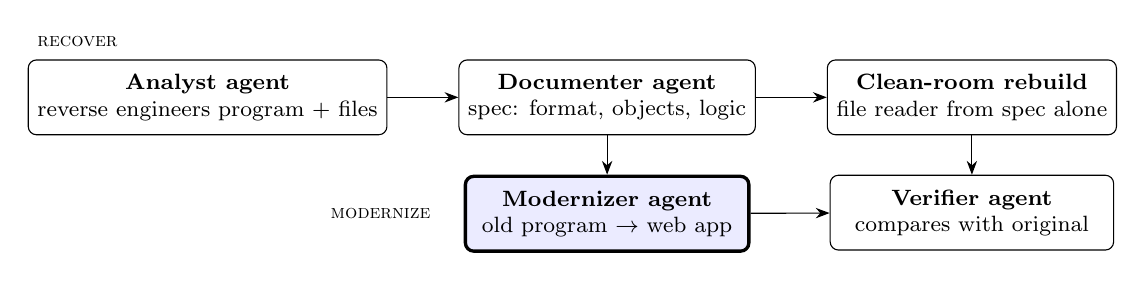
\begin{tikzpicture}[
  box/.style={draw, rounded corners=3pt, align=center, minimum width=3.6cm, minimum height=0.95cm, font=\footnotesize},
  main/.style={box, very thick, fill=blue!8},
  arr/.style={-{Stealth[length=5pt]}},
  node distance=0.5cm and 0.9cm]
  \node[box] (an) {\textbf{Analyst agent}\\reverse engineers program + files};
  \node[box, right=of an] (doc) {\textbf{Documenter agent}\\spec: format, objects, logic};
  \node[box, right=of doc] (cr) {\textbf{Clean-room rebuild}\\file reader from spec alone};
  \node[main, below=of doc] (mod) {\textbf{Modernizer agent}\\old program $\to$ web app};
  \node[box, below=of cr] (ver) {\textbf{Verifier agent}\\compares with original};
  \draw[arr] (an) -- (doc); \draw[arr] (doc) -- (cr);
  \draw[arr] (doc) -- (mod); \draw[arr] (mod) -- (ver); \draw[arr] (cr) -- (ver);
  \node[font=\scriptsize\scshape, anchor=east] at ([xshift=-0.3cm]mod.west) {modernize};
  \node[font=\scriptsize\scshape, above=1pt of an.north west, anchor=south west] {recover};
\end{tikzpicture}
\end{center}

\begin{enumerate}[label=\textbf{\arabic*.}]
  \item \textbf{Recover.} The analyst agent studies the program and its data files; the documenter
  turns the findings into a spec (file formats, object model, script behavior). A separate agent
  builds a file reader from the spec alone to test that it is accurate (clean-room approach).
  \item \textbf{Modernize.} The modernizer maps the program onto a modern architecture and translates
  its logic into readable code a person can edit. For HyperCard: cards become pages, fields become
  state, HyperTalk becomes JavaScript.
  \item \textbf{Verify.} The verifier runs the original in an emulator next to the modern version,
  repeats the same actions in both, and reports differences back to the modernizer.
\end{enumerate}

\sect{Evaluation}
Tested on HyperCard stacks of growing difficulty, then on a second program of a different kind:
\textbf{spec accuracy} (test files the clean-room reader opens correctly), \textbf{visual fidelity}
(screenshot comparison per screen), \textbf{behavioral fidelity} (scripted actions with the same
result in both), \textbf{maintainability} (can a person add a feature to the output), and
\textbf{generality} (how much of the pipeline carries over unchanged to the second program).

\sect{Scope and risks}
The deliverable is the reusable pipeline, proven on a few representative stacks (not every feature).
HyperTalk has many edge cases, so translation may stay partial; the fallback is reporting which
features convert reliably. Targets are limited to abandoned software or software whose license
allows analysis, and no original code is copied into the output.

\sect{Tools and prompt history}
Claude Code connected to a reverse-engineering MCP server (REA: decompilation, file-format analysis,
GDB/Frida instrumentation), plus emulators. All work runs from one project folder, so every session
transcript is saved under \texttt{\textasciitilde/.claude/projects/}; a \texttt{PROMPTS.md} log keeps
every prompt in English and marks the turns that changed the project's direction, for the presentation.

\end{document}
